\subsection{Lengths of Tracks}
\newthought{The most apparent difference } between the \href{box:MI}{two detection-methods } is the abundance of long-lived eddies resulting from the \MI-method. The major difference between the two methods is the way in which the \textit{shape} of found contour rings in SSH is decided to be sufficiently \textit{eddy-like} or not \TODO{hlink}.

\newthought{The } \MI-method is the more lenient one, as all it checks for, is whether the contour is of sufficiently compact form. The only shapes that are dismissed are long, thin elongated structures. This means that \eg an eddy-track can more easily \footnote{as long as the similarity-criterion is not violated.} survive situations in which two eddies merge into one or those in which one is split into two or situations in which mean current gradients distort the vortex.\\ There could also be the situation in which an old, weak eddy fades, yet another one emerges in sufficient proximity. These two events would not even have to be at the exact same time, as long as some short-lived coherent structure, of which there is an abundance at any given time-step throughout the world ocean, acted as a \textit{bridge} to fill the gap.

\newthought{The } \MII-method is conceptually different in that it is based on the assumption that a distinct coherent vortex need \textit{per definition} to be more or less circular. It will therefor be more likely to regard \eg the situation in which one eddy merges with another one as one of 3 eddies in total; \textbf{two} that have just died to create \textbf{one} new one.
The focus here is more on the propagation of distinct circular geostrophic vortices whereas the focus in the \MI-method is more general on coherent local depressions respective elevations in SSH. Unfortunately the time-frame of this work did not allow to test to which degree tracers \footnote{in the model data.} found within tracked eddies remained within the eddy over time. This could better clarify the assumption that the \MI-method may be better at tracking water-mass advecting entities, with less jumps between bodies of water.

\subsection{Scales}

\subsection{Drift Speeds}

\newthought{The } \MI detection method a priori assumes that an eddy is more or less detected at its asymptotic \textit{floor} \ie in the case of an anti-cyclone at the \textit{foot of the mountain}. The idea of the $\IQ$-based method on the other hand is to assume that the situation of a single well-defined eddy sitting on an otherwise smooth, flat sea surface, which would be necessary for the contour algorithm to find a closed contour describing the outermost perimeter of said single vortex, is unrealistic. Instead the approach is to look for distinct, sufficiently circular \textit{caps} of SSH- hills respepective valleys that consistently \textit{wade} through all other weaker geostrophic noise surrounding it. \TODO{ why gaussian or quad?}

\TODO{diff maps etc}

\begin{marginfigure}
		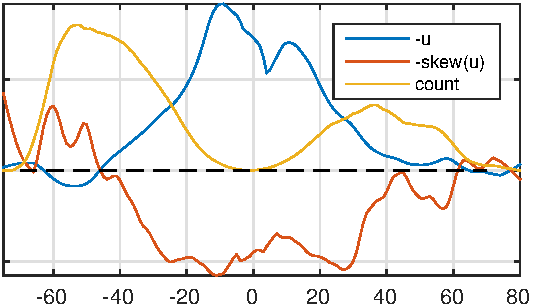
\includegraphics[]{Skew-aviI}
		\caption{TODO}
		\label{fig:SkewAviI}
\end{marginfigure}

\begin{marginfigure}
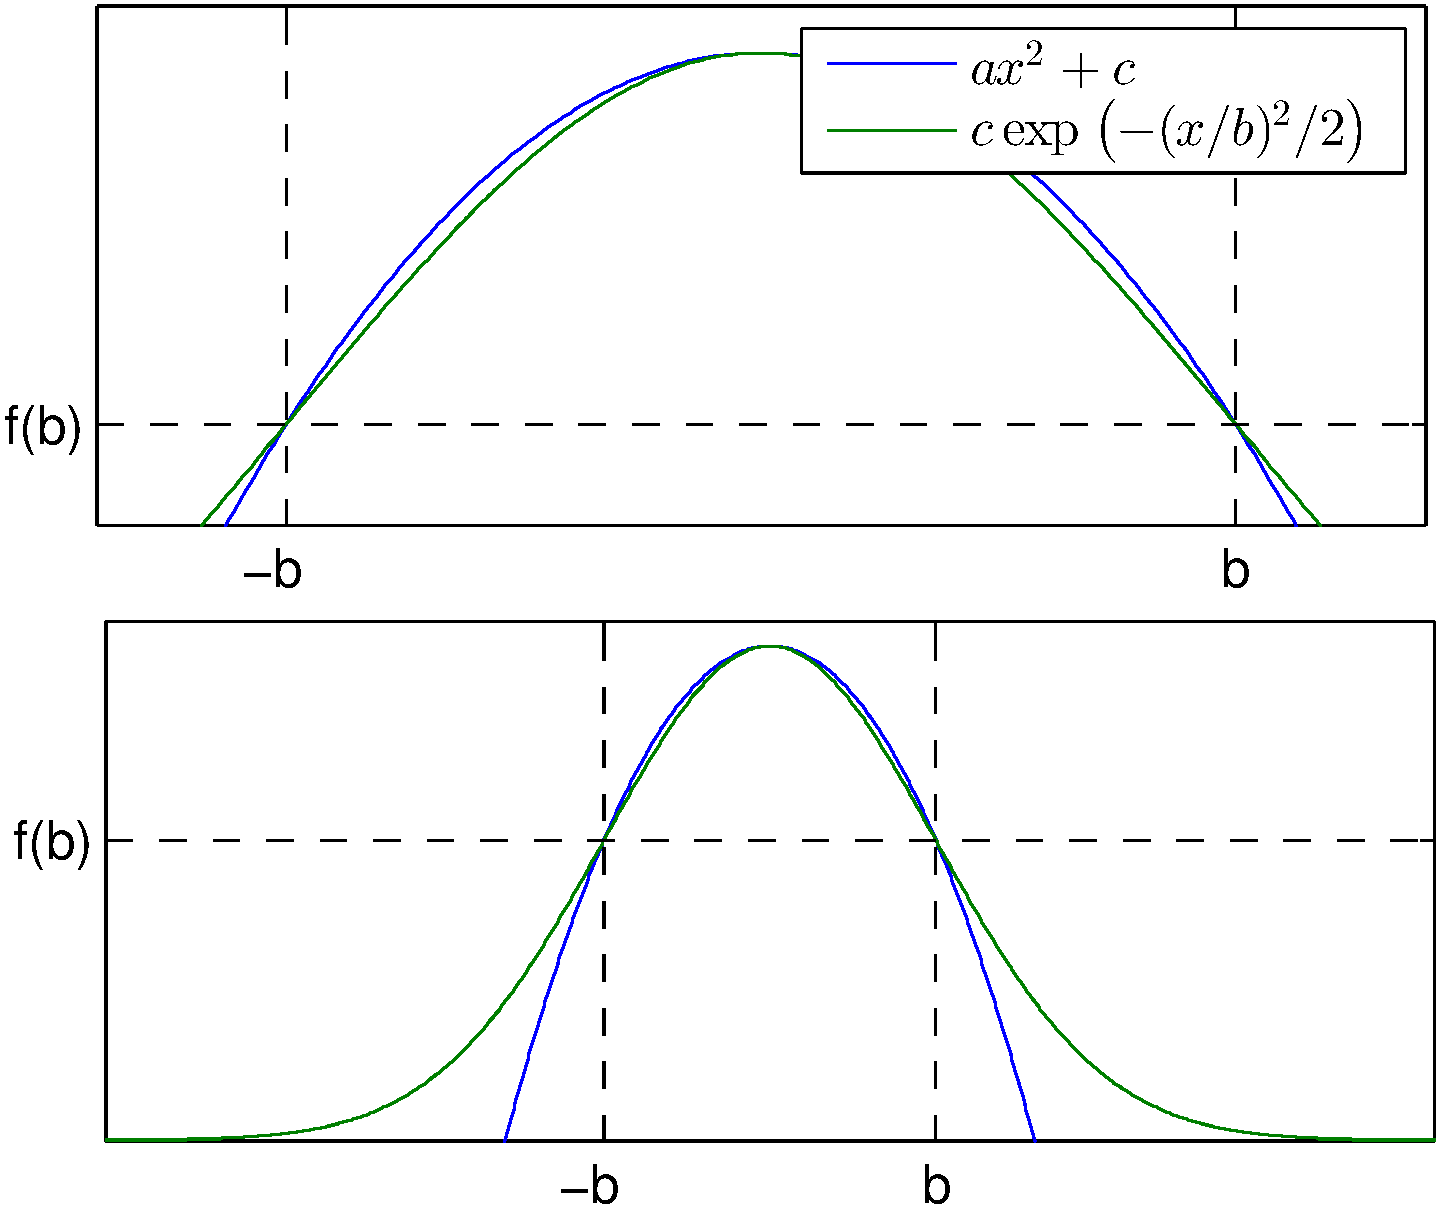
\includegraphics[]{gaussVSquadSmaller}
\caption{The upper part of a Gaussian profile can appear similar to a quadratic one.}
\label{fig:gaussVSquad}
\end{marginfigure}

%%....................................F.I.G.U.R.E.............................................
\begin{marginfigure}
	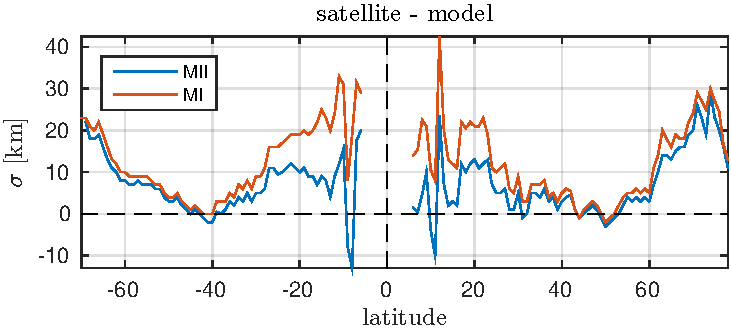
\includegraphics[]{sigmaSatMinusMod}
	\caption{\TODO{caption}}
	\label{fig:TODO}
\end{marginfigure}
%%....................................F.I.G.U.R.E.............................................
%%....................................F.I.G.U.R.E.............................................
\begin{marginfigure}
	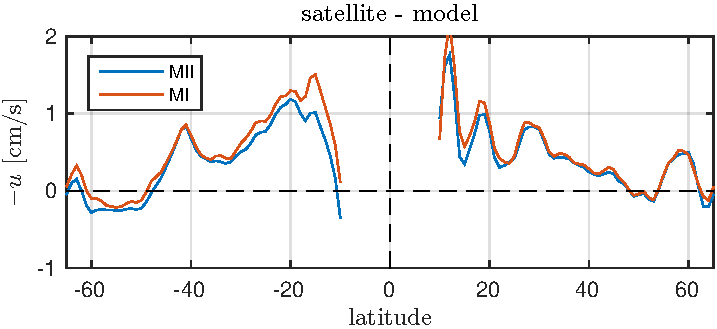
\includegraphics[]{velSatMinusMod}
	\caption{\TODO{caption}}
	\label{fig:TODO}
\end{marginfigure}
%%....................................F.I.G.U.R.E.............................................%%....................................F.I.G.U.R.E.............................................
\begin{marginfigure}
	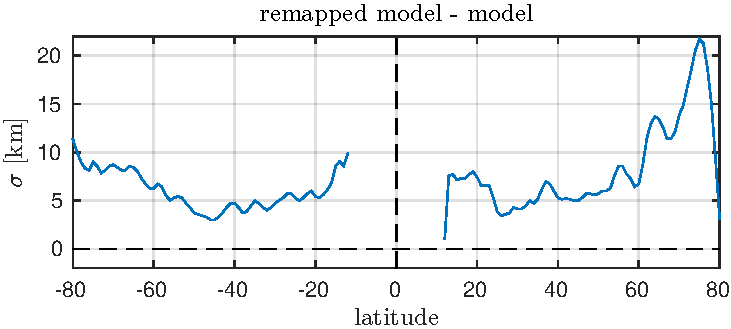
\includegraphics[]{sigmaP2aMinusMod}
	\caption{\TODO{caption}}
	\label{fig:TODO}
\end{marginfigure}
%%....................................F.I.G.U.R.E.............................................
